\begin{appendices}

\chapter{Lista defectelor din suită}
\label{apx:defecte}

\begin{figure}[h]
    \centering
    \caption{\centering Lista defectelor din suită (A)}
    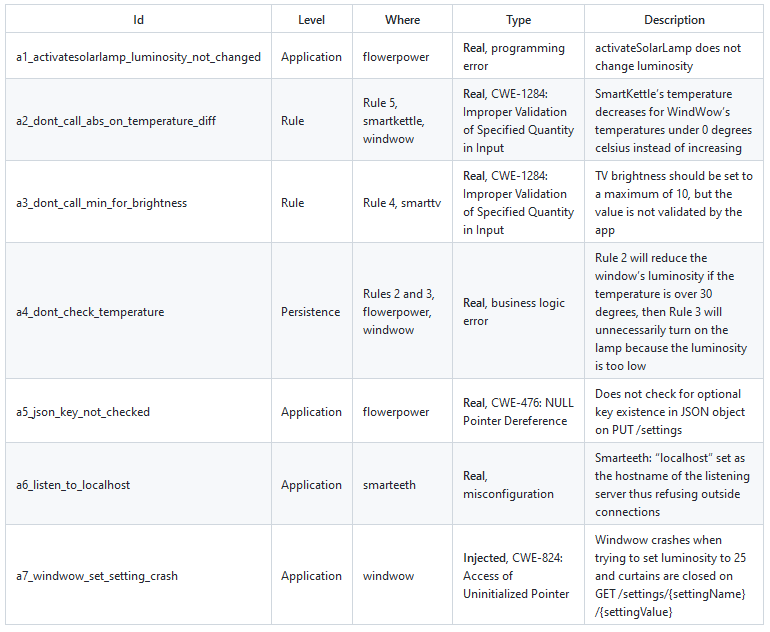
\includegraphics[width=0.9\textwidth]{images/tabel_bug2.png}
    \label{fig:tabel_bug1}
\end{figure}

\begin{figure}[h]
    \centering
    \caption{\centering Lista defectelor din suită (B)}
    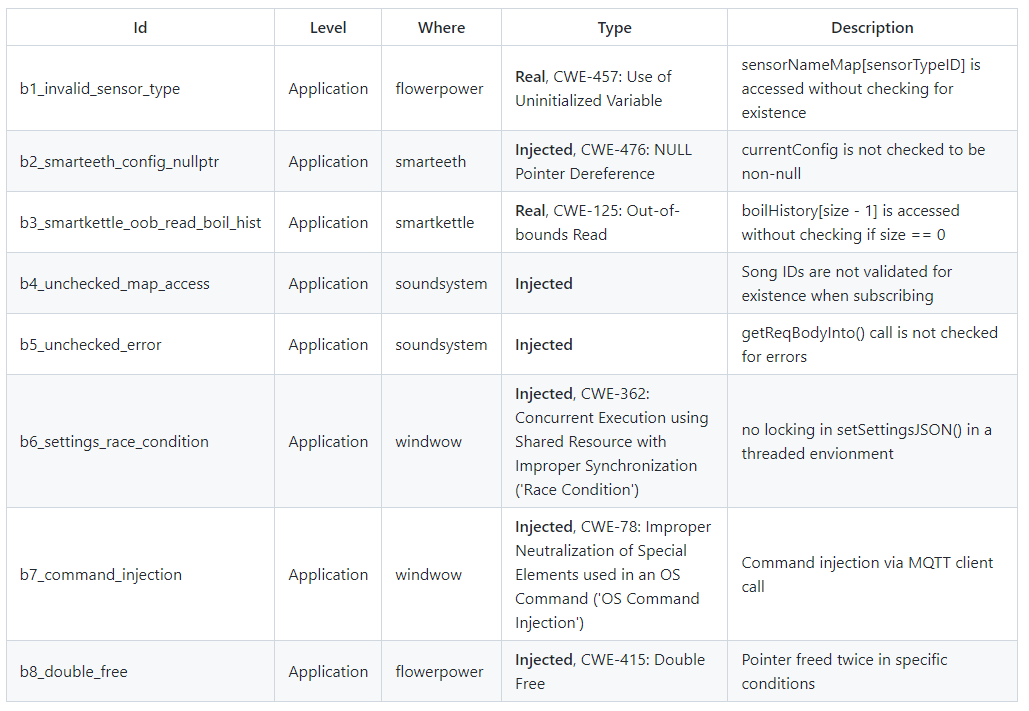
\includegraphics[width=0.9\textwidth]{images/tabel_bug1.png}
    \label{fig:tabel_bug2}
\end{figure}

\chapter{Ilustrații suplimentare}
\label{apx:ilustratii}

\begin{figure}[h]
    \centering
    \caption{\centering Modelul conceptual Open Systems Interconnection \newline (imagine prealuată de pe Wikipedia)}
    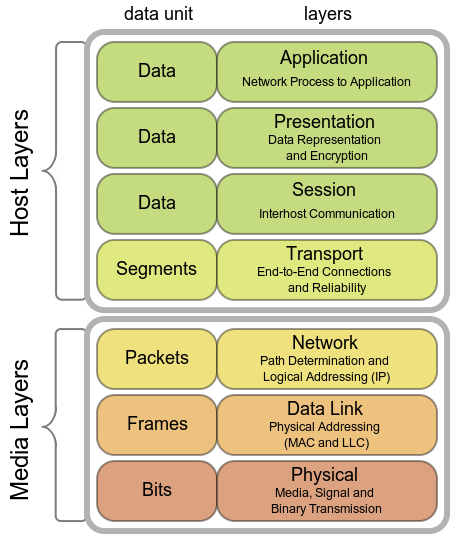
\includegraphics[width=0.8\textwidth]{images/OSI_Model_v1.png}
    \label{fig:osi_model}
\end{figure}

\begin{figure}[h]
    \centering
    \caption{Exemple de topologii ZigBee}
    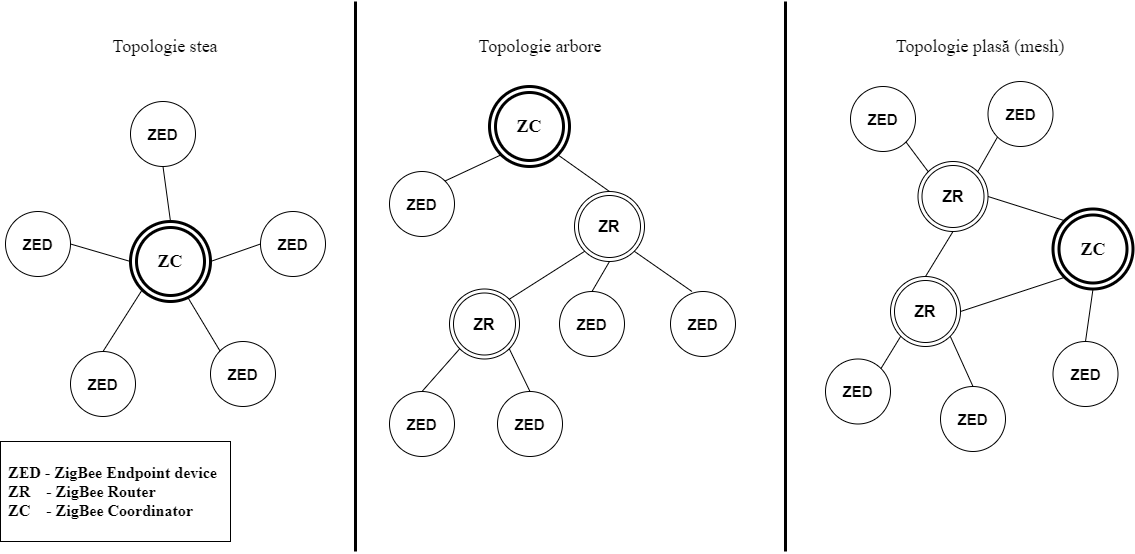
\includegraphics[width=0.9\textwidth]{images/topologii.drawio.png}
    \label{fig:zigbee_networks}
\end{figure}

\begin{landscape}
% Please add the following required packages to your document preamble:
% \usepackage{graphicx}
% \usepackage[table,xcdraw]{xcolor}
% If you use beamer only pass "xcolor=table" option, i.e. \documentclass[xcolor=table]{beamer}
\begin{table}[]
\centering
\resizebox{25cm}{!}{%
\begin{tabular}{|c|c|c|c|c|c|}
\hline
\rowcolor[HTML]{C0C0C0} 
\textbf{Tehnica de testare} &
  \textbf{Grad automatizare} &
  \textbf{Complexitate} &
  \textbf{Niveluri defecte} &
  \textbf{\begin{tabular}[c]{@{}c@{}}Procentaj defecte (cunoscute) detectate\\ (relativ la nivelurile relevante)\end{tabular}} &
  \textbf{Observații} \\ \hline
Testare funcțională BDD &
  Manual &
  Scăzută &
  Toate &
  Nu este relevant &
  \begin{tabular}[c]{@{}c@{}}Componentă exploratorie\\ insuficientă, bun pentru\\ scenarii pozitive\end{tabular} \\ \hline
Fuzzing cu RESTler &
  Automat &
  Medie &
  Aplicație, flux &
  TODO: ??? &
  \begin{tabular}[c]{@{}c@{}}Lipsa înțelegerii stării\\ aplicației, potrivit pentru\\ defecte de logică\end{tabular} \\ \hline
Analiză statică cu weggli &
  Parțial automat &
  Medie &
  Aplicație &
  ??? &
  \begin{tabular}[c]{@{}c@{}}Potrivit pentru defecte\\ de memorie\end{tabular} \\ \hline
Analiză statică cu cppcheck &
  Parțial automat &
  Scăzută &
  Aplicație &
  ??? &
  Rată mare de fals-pozitive \\ \hline
Verificare formală cu TLA+ &
  Parțial automat &
  Ridicată &
  Persistență &
  100\% &
  \begin{tabular}[c]{@{}c@{}}Potrivit pentru defecte\\ de concurență, necesită\\ cunoștințe matematice\end{tabular} \\ \hline
\end{tabular}%
}
\caption{Sumar comparativ al tehnicilor de testare abordate}
\label{tab:sumar_testare}
\end{table}
\end{landscape}

\chapter{Cod sursă suplimentar}
\label{apx:cod}

\begin{lstlisting}[caption={Specificația TLA+ a scenariului descris în capitolul 5, secțiunea despre verificare formală}, label={lst:tla_exemplu}]
----- MODULE light_example -----
EXTENDS Naturals, TLC

LightStates == {"on", "off"}
MotionStates == {"detected", "not detected"}
IsMidnight(x) == IF x % 5 = 0 THEN TRUE ELSE FALSE

\(\* --algorithm light\_example
variables 
    light\_state = "off", 
    motion\_state = "not detected",
    now = 1;

process motion\_sensor = 1
begin
A:
    while TRUE do
        with c\_state \in MotionStates do
            motion\_state := c\_state;
     
            if c\_state = "detected" then
                light\_state := "on";
            end if;
        end with;
    end while;
end process

process clock = 2
begin
B:
    while TRUE do
        now := now + 1;
    end while;
end process

process light\_timer = 3
begin
C:
    while TRUE do
        if IsMidnight(now) then
            light\_state := "off";
        end if;
    end while;
end process

end algorithm; *)
\* BEGIN TRANSLATION 
VARIABLES light\_state, motion\_state, now

vars == << light\_state, motion\_state, now >>

ProcSet == {1} \cup {2} \cup {3}

Init == \(\* Global variables *)
        /\ light\_state = "off"
        /\ motion\_state = "not detected"
        /\ now = 1

motion\_sensor == /\ \E c\_state \in MotionStates:
                      /\ motion\_state' = c\_state
                      /\ IF c\_state = "detected"
                            THEN /\ light\_state' = "on"
                            ELSE /\ TRUE
                                 /\ UNCHANGED light\_state
                 /\ now' = now

clock == /\ now' = now + 1
         /\ UNCHANGED << light\_state, motion\_state >>

light\_timer == /\ IF IsMidnight(now)
                     THEN /\ light\_state' = "off"
                     ELSE /\ TRUE
                          /\ UNCHANGED light\_state
               /\ UNCHANGED << motion\_state, now >>

Next == motion\_sensor \/ clock \/ light\_timer

Spec == Init /\ [][Next]\_vars

\* END TRANSLATION 

MotionLightValid == (motion\_state = "detected") => (light\_state = "on")

=========
\end{lstlisting}

\end{appendices}